\documentclass[a4paper]{article}
\usepackage{amsmath}
\usepackage{amsfonts}
\usepackage{amsthm}
\usepackage{amssymb}
\usepackage[english]{babel}
\usepackage{float}
\usepackage{graphicx}
\usepackage{hyperref}
\usepackage[utf8]{inputenc}
\usepackage{listings}
\usepackage{xcolor}
%% \usepackage{subfigure}
\usepackage{graphicx}
\usepackage{subcaption}
\usepackage{stmaryrd}

\usepackage{a4wide}
\usepackage{url}

\usepackage{appendix}

\graphicspath{{imgs/}} %Setting the graphicspath

\lstset{
  frame=tb,
  language=Python,
  aboveskip=3mm,
  belowskip=3mm,
  showstringspaces=false,
  formfeed=newpage,
  tabsize=4,
  comment=[l]{\#},
  breaklines=true,
  morekeywords={models, lambda, forms}
}

\newcommand{\prob}[1]{\mathbb{P}\left(#1\right)}
\newcommand{\expect}[1]{\mathbb{E}\left(#1\right)}
\newcommand{\avg}[1]{\sum_{i=1}^{#1}X_i}
\newcommand*{\QEDA}{\hfill\ensuremath{\blacksquare}}%

\newcommand{\bt}{\textbf}
\newcommand{\nt}{\text}
\newcommand{\lagr}{\mathcal{L}}
\newcommand{\isum}{\sum^\infty_}
\newcommand{\f}{$f$}

\title{\vspace{-5cm} Numerical Optimization \\ Re-exam Handin 1}
\author{Dmitry Serykh (qwl888)}

\begin{document}
%% \maketitle
%% \title{\Huge{\textbf{NO - Group Hand-In 1}}}
%% \author{Michael Emil Rosenstrøm (kfg364) \\ Magnus Fellenius-Blædel (gwm418) 
%% \\ Dmitry Serykh (qwl888) \\ Xuening He (pcr980)} 
\maketitle

\section{Introduction}
This submission based on the group handin
by myself, Michael Emil Rosenstrøm (kfg364), Magnus Fellenius-Blædel (gwm418),
and Xuening He (pcr980). In this assignment we will implement five case
functions including their gradients and hessians. The case functions are used to
test optimisation algorithms. We discuss how to test the case functions and show
results needed to perform an implementation of the functions.
%%% 

\section{Analysis}
%%% inserted from gwm418 report
\subsection{Testing of the case functions}
We can never test too much, so we we need to prioritize what to test. Finding
the local minima of a function is essential in minimisation problems. The five
case functions presented in this assignment are created to test optimization
algorithms. Therefore it is essential that implementations of the case function
are implemented correctly and especially that they have correct local minimum.

\subsection{Proof for the Diagonal Hessian Matrix}
For functions on the form $f(x) = \sum_{i=1}^N
g_i(x_i), x\in \mathbb{R}^N$ we have $(Hf(x))_{ii} = g_i''(x_i)$ we can spare
some time later in computing the Hessian of functions like the ellipsoid
function and the attractive sector functions. \\\\
$\frac{\partial f(x)}{\partial x_i} = g_i'(x_i)$ because all $\frac{\partial g_j(x_j)}{\partial x_i}=0,j\neq i$ as they do not depend on $x_i$ and
\begin{align*}
  \frac{\partial f(x)}{\partial x_i \partial x_j} =   \left\{
  \begin{array}{ll}
    g_i''(x_i) \hspace*{5mm}  & i=j\\
    0                        & i\neq j
  \end{array}
  \right.
\end{align*}
as all $\frac{\partial g_i(x_i)}{\partial x_i \partial x_j}=0,j\neq i$ as they do not depend on $x_j$.

\section{The Ellipsoid function}
The Ellipsoid function is defined as
\begin{align*}
  f_1(x) = \sum_{i=1}^d \alpha^{\frac{i-1}{d-1}} x_i^2
\end{align*}
and has gradient
\begin{align*}
  (\nabla f_1(x))_i = 2\alpha^{\frac{i-1}{d-1}} x_i
\end{align*}
and Hessian
\begin{align*}
  (Hf_1(x))_{ij} =
  \left\{
  \begin{array}{ll}
    2 \alpha^{\frac{i-1}{d-1}} \hspace*{5mm}  & i=j\\
    0                                     & i\neq j
  \end{array}
  \right.
\end{align*}
The following 3d plot and contour plot gives an idea of the shape of the Ellipsoid funtion 
\begin{figure}[h]
    \centering
    \subfloat[3d plot]{{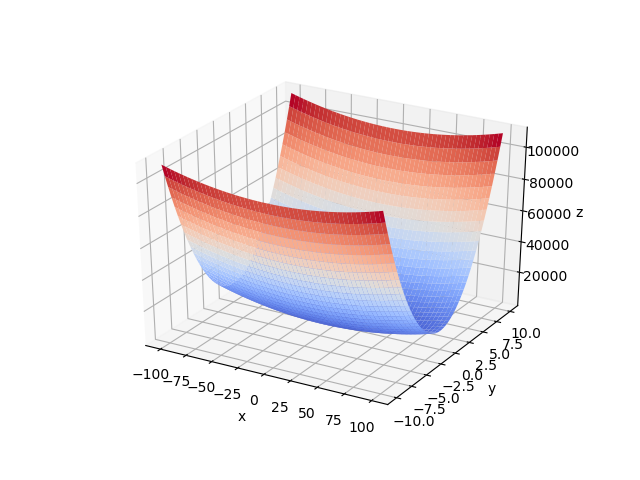
\includegraphics[width=6cm]{plt11.png} }}%
    \qquad
    \subfloat[Contour plot]{{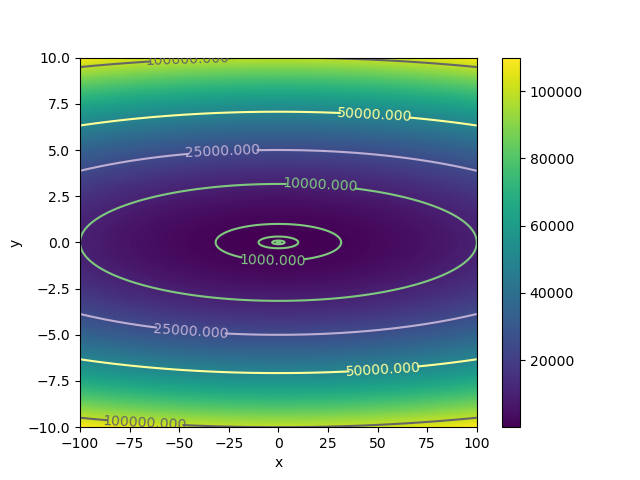
\includegraphics[width=6cm]{plt12.png} }}%
    \caption{These two figures of the ellipsoid function demonstrates the local minimum of the function}%
    \label{fig:1}%
\end{figure}\\
The gradient at (0,0) is given by
\begin{align*}
  (\nabla f_1(0,0))_i = 2\alpha^{\frac{i-1}{d-1}} 0 = 0 
\end{align*}
as $f_1$ is continously differentiable in a neighborhood of (0,0) and $(\nabla f_1(0,0))_i = \bt{0}$, (0,0) is a local minimizer according to theorem 2.2. The Hessian in (0,0) is given by
\begin{align*}
  (Hf_1(0,0))_{ij} =
  \left\{
  \begin{array}{ll}
    2 \alpha^{\frac{i-1}{d-1}} \hspace*{5mm}  & i=j\\
    0                                     & i\neq j
  \end{array}
  \right.
\end{align*}
and we can clearly see without computation that both det$(Hf_1(0,0))>0$ and trace$(Hf_1(0,0))>0$ and thus $Hf_1(0,0)$ is positive definite. Since $(\nabla^2 f_2(x))_i$ is continous and we just found that $(\nabla f_1((0,0)))_i = \bt{0}$ we have according to 2.4 that (0,0) is a strict local minimizer, which is in good accordance with the ellipsoid plot.


\section{The Rosenbrock Banana Function}
The Rosenbrock banana function is defined as
\begin{align*}
  f_2(x) = (1-x_1)^2 + 100(x_2-x_1^2)^2
\end{align*}
and has gradient
\begin{align*}
  (\nabla f_2(x))_i =
  \begin{pmatrix}
    -2(1-x_1)-400x_1(x_2-x_1^2)\\
    200(x_2-x_1^2)
   \end{pmatrix}
\end{align*}
and Hessian
\begin{align*}
  (Hf_2(x)) =
  \left(
  \begin{array}{cc}
    2-400x_2+1200x_1^2 & -400x_1\\
    -400x_1           &  200
  \end{array}
  \right)
\end{align*}
The following 3d plot and contour plot gives an idea of the shape of the Rosenbrock banana funtion 
\begin{figure}[h]
    \centering
    \subfloat[3d plot]{{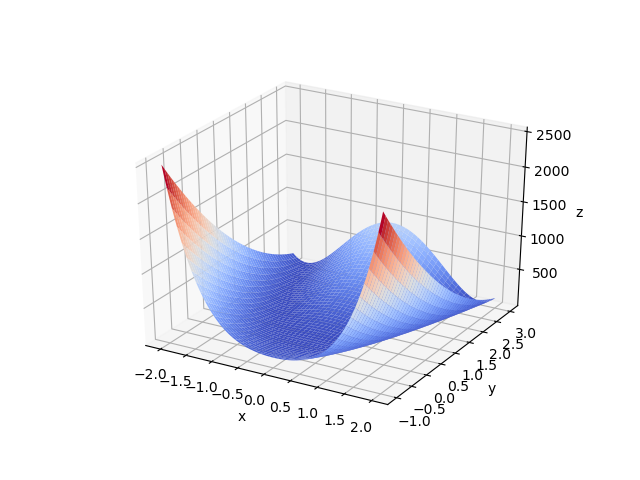
\includegraphics[width=6cm]{plt21.png} }}%
    \qquad
    \subfloat[Contour plot]{{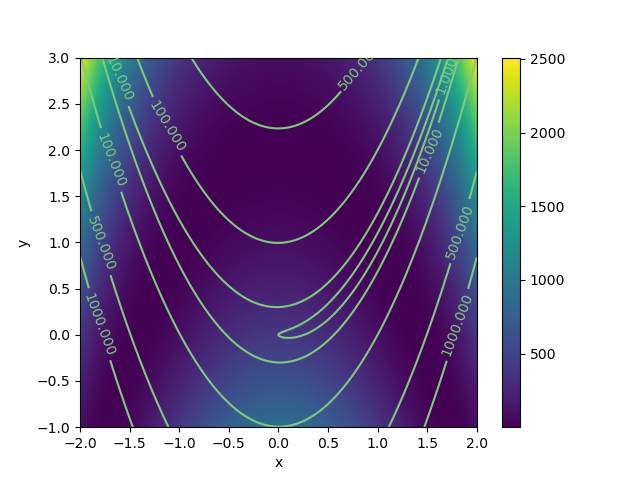
\includegraphics[width=6cm]{plt22.png} }}%
    \caption{The plots show the Rosenbrock banana function. The point (1,1) is a strict local minimizer  of the function. On plot b the point (1,1) can be seen in the lowest level.}%
    \label{fig:2}%
\end{figure}

The gradient in (1,1) is given by
\begin{align*}
  (\nabla f_2((1,1)))_i =
  \begin{pmatrix}
    -2(1-1)-400(1-1^2)\\
    200(1-1^2)
  \end{pmatrix} =
  \begin{pmatrix}
    0\\
    0
  \end{pmatrix}
\end{align*}
as $f_2$ is continously differentiable in a neighborhood of (1,1) and $(\nabla f_2((1,1)))_i = \bt{0}$, (1,1) is a local minimizer according to theorem 2.2. The Hessian in (1,1) is given by
\begin{align*}
  (Hf_2(1,1)) =
  \left(
  \begin{array}{cc}
    2-400+1200 & -400\\
    -400       &  200
  \end{array}
  \right)=
  \left(
  \begin{array}{cc}
    802  & -400\\
    -400 &  200
  \end{array}
  \right)
\end{align*}
with det$((Hf_2(1,1)))=400$ and trace$((Hf_2(1,1)))=1002$. Since det$((Hf_2(1,1)))>0$ and trace$((Hf_2(1,1)))>0$ we know that $(Hf_2(1,1))$ is positive definite and as $(\nabla^2 f_2(x))_i$ is clearly continous in an open interval of (1,1) and we found before that $(\nabla f_2((1,1)))_i = \bt{0}$, (1,1) is a strict local minimizer according to theorem 2.4.

\section{The Log-Ellipsoid function}
The log-Ellipsoid function is defined as
\begin{align*}
  f_3(x) = \log(\epsilon-f_1(x)), \hspace*{10mm} \epsilon=10^{-16}
\end{align*}
and has gradient
\begin{align*}
  (\nabla f_3(x))_i = \frac{2\alpha^{\frac{i-1}{d-1}}x_i}{\epsilon + \sum_{i=1}^d \alpha^{\frac{i-1}{d-1}}x_i^2}
\end{align*}
and Hessian
\begin{align*}
  (Hf_3(x))_{ij} = -\frac{4\alpha^{\frac{i-1}{d-1}}\alpha^{\frac{j-1}{d-1}}x_ix_j}{(\epsilon + \sum_{i=1}^d \alpha^{\frac{i-1}{d-1}}x_i^2)^2}
\end{align*}
The following plot gives in idea of the shape of the Log-ellipsoid function
\begin{figure}[h]
    \centering
    \subfloat[3d plot]{{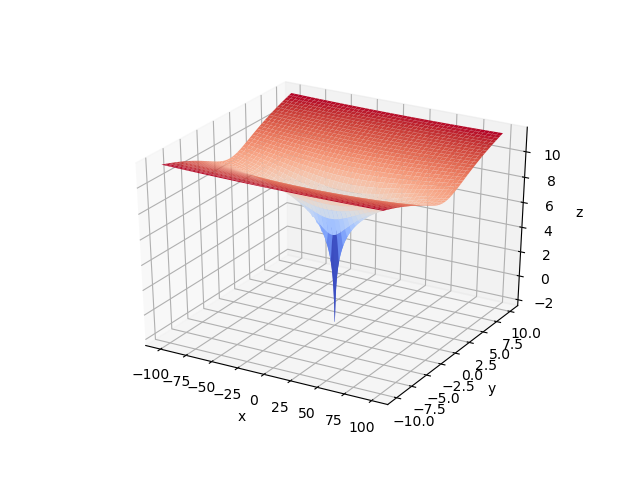
\includegraphics[width=6cm]{plt31.png} }}%
    \qquad
    \subfloat[Contour plot]{{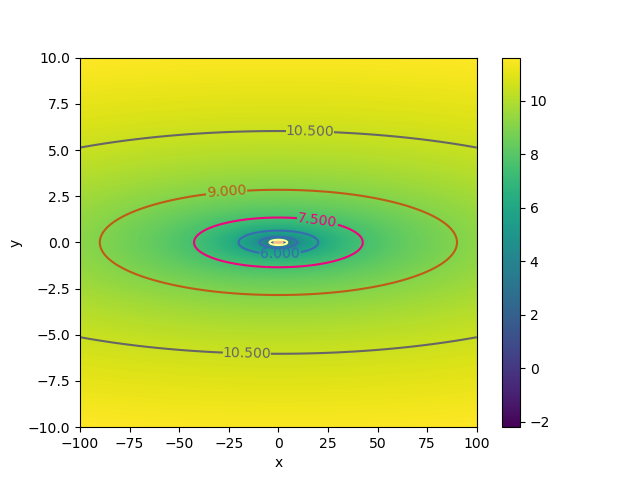
\includegraphics[width=6cm]{plt32.png} }}%
    \caption{The plots show that the point (0,0) is a strict local minimizer for the log-Ellipsoid function}%
    \label{fig:3}%
\end{figure}


\section{The Attractive-Sector Functions}
The Attractive-Sector planar function is defined as
\begin{align*}
  f_4(x) = \sum_{i=1}^d h(x_i) + 100h(-x_i), \hspace*{10mm} h(x) = \frac{\log(1+\exp(qx))}{q},\ q=10^8
\end{align*}
and it has gradient
\begin{align*}
  (\nabla f_4(x))_i = \frac{\exp(qx_i)}{1+\exp(qx_i)}-100\frac{\exp(-qx_i)}{1+\exp(-qx_i)}
\end{align*}
and Hessian
\begin{align*}
  (Hf_4(x))_{ij} =
    \left\{
  \begin{array}{ll}
    \frac{\exp(qx_i)}{(1+\exp(qx_i))^2}+100\frac{\exp(-qx_i)}{(1+\exp(-qx_i))^2} \hspace*{5mm}  & i=j\\
    0                                     & i\neq j
  \end{array}
  \right.
\end{align*}
Before we start programming and ploting it is worth noting that
\[
\log(1+\exp(x)) = \log(1+\exp(-|x|))+\max(x,0)
\]
since:
\begin{align*}
  \begin{array}{lcl}
    \text{for } x<0:\\
    \log(1+\exp(-x)) &=& \log(1+\exp(-|-x|))+\max(-x,0)\\
    &=& \log(1+\exp(-x))+0\\
    &=& \log(1+\exp(-x))\\
    \text{for } x\geq 0:\\
    \log(1+\exp(x)) &=& \log(1+\exp(-x))+\max(x,0)\\
    &=& \log(1+\exp(-x))+x\\
    &=& \log(1+\exp(-x))+\log(\exp(x))\\
    &=& \log((1+\exp(-x))\exp(x))\\
    &=& \log((1+\exp(-x))\exp(x))\\
    &=& \log(1+\exp(x))\\
  \end{array}
\end{align*}
This formulation is beneficial in a context of a computer implementation, since when x is a large
number, such as $10^8$ in the Attractive-Sector function. The value of e x would be a huge number
that is much larger than $10^{32}$ or even $10^{64}$ . Therefore, it can not fit in any type of CPU registers
and would result in a overflow. $|x|> 0$ for all real values of $x$, hence $e^{-|x|}$ would become a
very small number for high values of $x$ and would be rounded to zero, which would eliminate the
overflow problem.

\begin{figure}[h]
    \centering
    \subfloat[3d plot]{{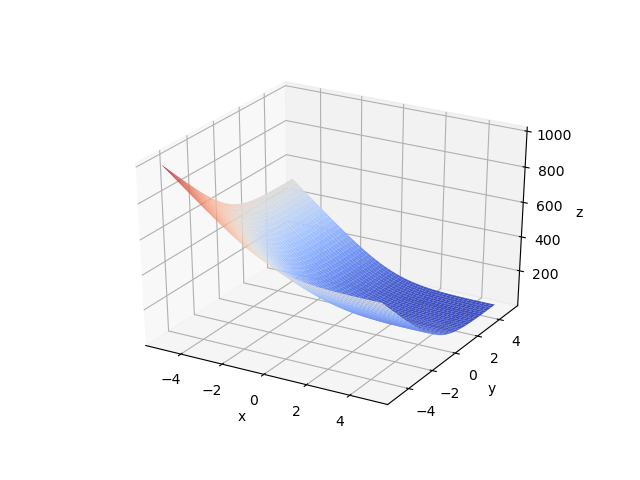
\includegraphics[width=6cm]{plt41.png} }}%
    \qquad
    \subfloat[Contour plot]{{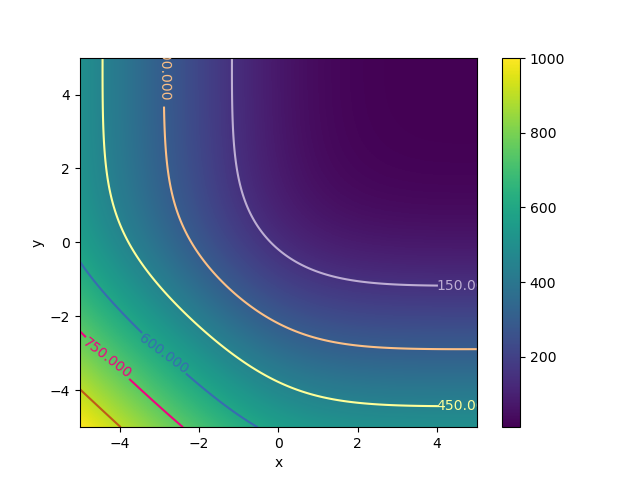
\includegraphics[width=6cm]{plt42.png} }}%
    \caption{The plots show the surface of the Attractive Sector planar function}%
    \label{fig:4}%
\end{figure}
The Attractive-Sector quadratic function is defined as
\begin{align*}
  f_5(x) = \sum_{i=1}^d h(x_i)^2 + 100h(-x_i)^2, \hspace*{10mm} h(x) = \frac{\log(1+\exp(qx))}{q},\ q=10^8
\end{align*}
and it has gradient
\begin{align*}
  (\nabla f_5(x))_i = \frac{2\log(1+\exp(qx_i))\exp(qx_i)}{q(1+\exp(qx_i))}-\frac{2\log(1+\exp(-qx_i))\exp(-qx_i)}{q(1+\exp(-qx_i)}
\end{align*}
and Hessian
\begin{align*}
  (Hf_5(x))_{ij} = 
  \left\{
  \begin{array}{ll}
    \frac{2\exp(qx_i)(\log(1+\exp(qx_i))+\exp(qx_i))}{(1+\exp(qx_i))^2}+\frac{2\exp(-qx_i)(\log(1+\exp(-qx_i))+\exp(-qx_i))}{(1+\exp(-qx_i)^2}
    \hspace*{5mm}  & i=j\\
    0                                     & i\neq j
  \end{array}
  \right.
\end{align*}
The following 3d and contour plot gives an idea of the shape of the attractive sector quadratic function, which looks a lot like $f_4$ but but is curved where $f_4$ seems to have sharp edges. 
\begin{figure}[h]
    \centering
    \subfloat[3d plot]{{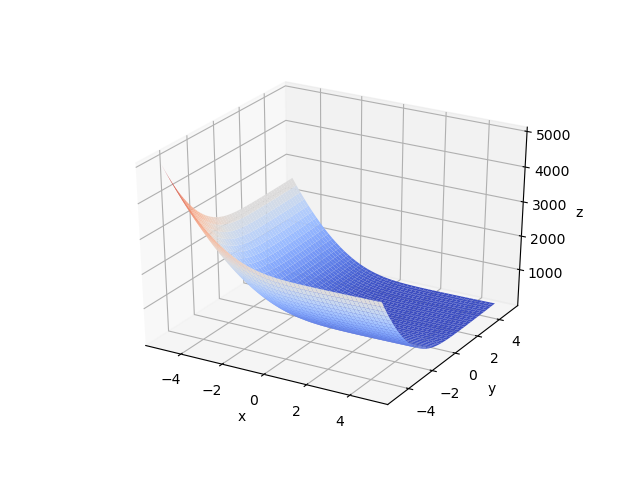
\includegraphics[width=6cm]{plt51.png} }}%
    \qquad
    \subfloat[Contour plot]{{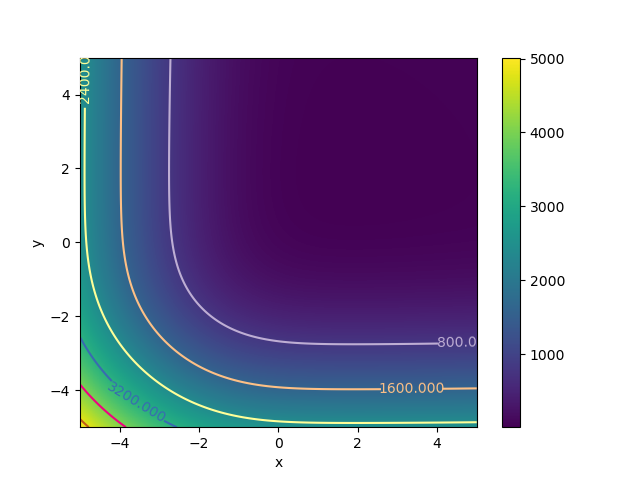
\includegraphics[width=6cm]{plt52.png} }}%
    \caption{The plots show the surface of the Attractive-Sector quadratic function}%
    \label{fig:5}%
\end{figure}
 
\section{Testing Protocol} 
In order to test if our calculation of gradient is correct, we can test if it
equals 0 at the optima of the functions, which is $(1,1)$ for the Rosenbrock
function and $(0,0)$ for the others.

\section{Conclusion} 
In this assignment we have implemented the five case functions and their gradient and hessian. We have tested that our implementations performs correct in local minimas of the functions. Our tests show that the five case functions are implemented correctly.
\end{document}

